\documentclass[page number]{beamer}
\usetheme[sectionpage=none,numbering=fraction,progressbar=foot]{metropolis}
\usepackage{etex}
\usepackage{graphicx, booktabs} % For tabulars
\usepackage{pgf,tikz}
\usepackage{ulem}
\usetikzlibrary{arrows}
\usetikzlibrary{positioning,shapes,fit}
\usepackage{algorithm}
\usepackage{algpseudocode}
\usepackage{multicol}
\usepackage{syntax}
\usepackage{xcolor, color, colortbl}
\usepackage{tikz-qtree}
\usepackage{listings}
\usepackage{mathtools}
\usepackage{amssymb}
\usepackage{amsmath}

\makeatletter
\makeatother

%\setcounter{tocdepth}{1} % remove subsection from table of contents

% colors
\definecolor{mDarkRed}{HTML}{6F1616}
\definecolor{mDarkGreen}{HTML}{106235}
\definecolor{mTeal}{HTML}{112233}
\definecolor{mBlack}{HTML}{000000}
\setbeamercolor{normal text}{fg=mTeal}
\setbeamercolor{alerted text}{fg=mDarkRed}
\setbeamercolor{example text}{fg=mDarkGreen}
\setbeamercolor{title separator}{fg=purple,bg=mBlack}

% macros
\def\ctls{CTL$^{*}$}
\def\ctlskd{CTL$^{*}$K$\Delta$}
\def\ctlskdp{CTL$^{*}$K$\Delta\psi$}
\def\ap{AP}
\def\A{\mathit{A}}
\def\E{\mathit{E}}
\def\U{\mathit{U}}
\def\R{\mathit{R}}
\def\X{\mathit{X}}
\def\K{\mathit{K}}
\def\KP{\bar{\mathit{K}}}
\def\D#1{\Delta^{#1}}
\def\eq#1#2{\approx^{#2}_{#1}}
\def\eqh#1{\approx_{#1}}
\def\eqstate#1{\sim_{#1}}
\def\todo#1{{\color{red}#1}}
\def\iff{\ \mathit{iff}\ }
\def\UD{U_{\Delta}}
\def\UT{U_T}
\def\UDK#1{U_{\Delta #1}}
\def\UTK#1{U_{T #1}}
\def\FV{\mathit{FH}}
\def\FP{\mathit{FP}}
\def\ktree{$k$-tree}
\def\ktrees{$k$-trees}
\def\outline{
  \begin{frame}[plain,noframenumbering]
    \frametitle{Outline}
    \tableofcontents[currentsection]
  \end{frame}
}


\begin{document}
\title[\ctlskd]{Defining and Model-Checking an Epistemic Temporal Logic with Changes of Observations}

\author[Aur\`ele Barri\`ere]{Aur\`ele Barri\`ere\hfill\textbf{Supervisors:}\begin{tabular}{c}
    Aniello Murano\\
    Bastien Maubert\\
    Sasha Rubin\\
  \end{tabular}}
% add supervisors
\date{\textit{ENS Rennes\hfill Universit\`a degli Studi di Napoli Federico II}
  \vfill
  \textbf{January 8, 2018}}

\def\outline{
  \begin{frame}[plain,noframenumbering]
    \frametitle{Outline}
    \tableofcontents[currentsection]
  \end{frame}
}

\begin{frame}[plain,noframenumbering]
  \vspace{-2cm}
  \maketitle
  \vspace{-4cm}
\end{frame}

\metroset{sectionpage=none}
\section{Introduction}
\begin{frame}{Temporal Logics}

  \begin{block}{Evolving Systems}
    Typically modelled wih \textbf{Kripke Structures} $M=(S,I,T,V)$.\\

    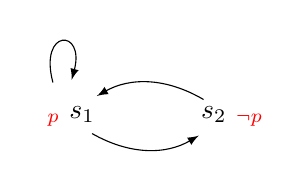
\begin{tikzpicture}[%
        every node/.style={circle,minimum size=4pt,minimum height=4pt, inner sep=0pt},
        shorten >=2pt,
        node distance=1.3cm, >=latex
      ]
      \node [] (0) [circle] {$~_{\color{red}~ p}~s_{1}$};
      \node [] (1) [circle, right=of 0] {$s_{2}~_{\color{red}\neg p}$}; 
      \path [draw] (0) edge[->, bend right]  node {} (1)
      (0) edge[->, loop above]  node {} (0)
      (1) edge[->, bend right]  node {} (0);
    \end{tikzpicture}\hfill
    \begin{tabular}{c l l}
      $S$ & States &\\
      $I$ & Initial states & $\subseteq S$\\
      $T$ & Transitions & $\subseteq S\times S$\\
      $V$ & Valuation & $S\rightarrow 2^{AP}$
    \end{tabular}
  \end{block}
  \vfill
  \begin{block}{Temporal Logics}
    \begin{tabular}{l c r}
    Syntax & defines & $\varphi$\\
    Semantics & defines & $M\models\varphi$
    \end{tabular}
  \end{block}
  \vfill
  \begin{block}{Model-Checking}
    Given Kripke Structure $M$, and formula $\varphi$, does $M\models\varphi$?
  \end{block}
  
\end{frame}


\begin{frame}{A Temporal Logic: \ctls}

  \begin{block}{Syntax}
    \begin{tabular}{l l}
      State formulas & $\varphi := p ~|~ \neg \varphi ~|~ \varphi\wedge\varphi ~|~ \A\psi$\\
      Path formulas & $\psi := \varphi ~|~ \neg\psi ~|~ \psi\wedge\psi ~|~ \X\psi ~|~ \psi\U\psi$\\
    \end{tabular}
    
      $\A:$ for all paths\hfill
      $\X:$ next\hfill
      $\U:$ until\hfill
  \end{block}
  \vfill
  \begin{block}{Semantics}
    \begin{tabular}{l c l}
      $M,s \models p $&$ \iff $&$ p\in V(s)$\\
      $M,s \models \A\psi  $&$ \iff $&$ \forall\pi$ that starts in $s$, we have $M,\pi\models\psi$\\
      $M,\pi\models\varphi $&$ \iff $&$ M,\mathit{last}(\pi)\models\varphi$\\
      $M,\pi\models\X\psi $&$ \iff $&$  M,\pi_{> 0}\models\psi$\\
      $M,\pi\models\psi_1\U\psi_2 $&$ \iff $&$ \exists m\geq 0$ such that $\forall k\in[0,m[, M,\pi_{\geq k}\models\psi_1$\\
          & & and $M,\pi_{\geq m}\models\psi_2$\\
          \hline
      $M\models\varphi$&$ \iff $&$\forall s\in I, \quad M,s\models\varphi$
\end{tabular}
  \end{block}
  
\end{frame}


\begin{frame}{Model Checking}

  \begin{block}{Exemple}
    \begin{center}
     \begin{tikzpicture}[%
        every node/.style={circle,minimum size=4pt,minimum height=4pt, inner sep=0pt},
        shorten >=2pt,
        node distance=0.6cm, >=latex
      ]
      \node [] (0) [circle] {$s_{1}$};
      \node [] (1) [circle, below right=of 0] {$s_{2}$};
      \node [] (2) [circle, below left=of 0] {$s_{3}$};
      \node [] (3) [circle, below right=of 2] {$s_{4}~_{\color{red}p}$};
      \node [] (4) [circle, above=of 0] {};
      \node [] (5) [rectangle, right=of 1,xshift=1cm] {$\varphi=\A\X\X p$};      
      \path [draw] (0) edge[->]  node {} (1)
      (1) edge[->]  node {} (3)
      (0) edge[->]  node {} (2)
      (2) edge[->]  node {} (3)
      (4) edge[->]  node {} (0);
     \end{tikzpicture}
    \end{center}
     For every possible path starting in $s_1$, $p$ is true after two steps.
  \end{block}
  \vfill
  \begin{exampleblock}{Model Checking of \ctls\ is decidable}
    Complexity PSPACE.
  \end{exampleblock}
  
\end{frame}


\begin{frame}{Epistemic Logics}

  \begin{block}{Multi-agent systems and Imperfect Information}
    Agents each have an observation (equivalence relation on states).
    \vspace{-0.4cm}
    \begin{center}
    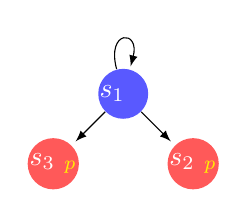
\begin{tikzpicture}[%
        every node/.style={circle,minimum size=4pt,minimum height=4pt, inner sep=0pt},
        shorten >=2pt,
        node distance=0.6cm, >=latex
      ]
      \node [] (0) [circle, fill=blue!65] {$\color{white}s_{1}~_{\hphantom{p}}$};
      \node [] (1) [circle, below right=of 0, fill=red!65] {$\color{white}s_{2}~_{\color{yellow}p}$};
      \node [] (2) [circle, below left=of 0, fill=red!65] {$\color{white}s_{3}~_{\color{yellow}p}$};
      \path [draw] (0) edge[->]  node {} (1)
      (0) edge[->, loop above]  node {} (0)
      (0) edge[->]  node {} (2);
    \end{tikzpicture}
    \quad\quad\quad
    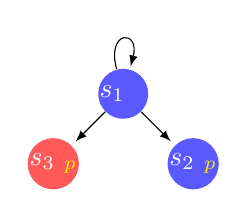
\begin{tikzpicture}[%
        every node/.style={circle,minimum size=4pt,minimum height=4pt, inner sep=0pt},
        shorten >=2pt,
        node distance=0.6cm, >=latex
      ]
      \node [] (0) [circle, fill=blue!65] {$\color{white}s_{1}~_{\hphantom{p}}$};
      \node [] (1) [circle, below right=of 0, fill=blue!65] {$\color{white}s_{2}~_{\color{yellow}p}$};
      \node [] (2) [circle, below left=of 0, fill=red!65] {$\color{white}s_{3}~_{\color{yellow}p}$};
      \path [draw] (0) edge[->]  node {} (1)
      (0) edge[->, loop above]  node {} (0)
      (0) edge[->]  node {} (2);
    \end{tikzpicture}
    \end{center}
    \vspace{-0.4cm}    
  \end{block}
  \vfill
  \begin{block}{Knowledge operator}
    \begin{tabular}{r l}
      $\K_a p$ : & Agent $a$ knows that $p$ holds.\\
      $\K_a\K_b p$ : & Agent $a$ knows that agent $b$ knows $p$.
    \end{tabular}
  \end{block}
  \vfill
  \begin{exampleblock}{Epistemic Temporal Logics}
    System goes through $(s_1,s_2)$.\\
    \begin{tabular}{l l}
    Possible histories for & agent 1: $(s_1,s_2)$ and $(s_1,s_3)$.\\
                           & agent 2: $(s_1,s_2)$ and $(s_1,s_1)$.
    \end{tabular}\\
    Only the first agent knows that $p$ holds.
  \end{exampleblock}
  
\end{frame}


\begin{frame}{Strategy Logic with Imperfect Information}

  \begin{block}{A logic for strategies in multi-agent systems}
    $\left<\left< x\right>\right>^o~(a,x)~\varphi$~:\quad
    There exists a strategy $x$ with observation $o$, such that if agent $a$ uses $x$, $\varphi$ holds.
  \end{block}
  \vfill
  \begin{alertblock}{Changes of observation}
    $\left<\left< x\right>\right>^o\left<\left< y \right>\right>^{o'}~(a,x)~\X~(a,y)~\varphi$
  \end{alertblock}
  \vfill
  \begin{exampleblock}{Towards an epistemic extension of SLii}
    How do changes of observations and epistemic operators interact?
  \end{exampleblock}
    
\end{frame}


\begin{frame}{\ctlskd}

  \begin{block}{An Epistemic Temporal Logic with Changes of Observation}
    \begin{itemize}
    \item Branching-time Temporal Operators $\X,\U,\A$.
    \item Knowledge Operator $\K$.
    \item Dedicated operator for change of observation $\D{o}$.
    \item Synchronous Perfect-Recall Semantics.
    \end{itemize}
  \end{block}
  \vfill
  \begin{exampleblock}{Objectives}
    \begin{itemize}
    \item Define \ctlskd\ for the single-agent setting.
    \item Solve the model-checking problem.
    \item Extend logic and model-checking to the multi-agent setting.
    \end{itemize}
  \end{exampleblock}
  
\end{frame}


\metroset{sectionpage=progressbar}
\section{\ctlskd: Single Agent}
\begin{frame}{\ctlskd\quad Syntax}

  \begin{block}{Syntax}
    \begin{tabular}{r l}
    History Formula: & $\varphi := p ~|~ \neg \varphi ~|~ \varphi\wedge\varphi ~|~ \A\psi ~|~$\color{red!85!blue}$ \K\varphi ~|~ \D{o}\varphi$\\
    Path Formula: & $\psi := \varphi ~|~ \neg\psi ~|~ \psi\wedge\psi ~|~ \X\psi ~|~ \psi\U\psi$
    \end{tabular}
  \end{block}
  \vfill
  \begin{block}{Definitions}
    History: finite sequence of states.\\
    Path: infinite sequence of states.
  \end{block}
  
\end{frame}


\begin{frame}{\ctlskd\quad Models}

  \begin{block}{Kripke Structures with Observations}
    $AP$ atomic propositions.
    $\mathcal{O}$ set of $m$ observations.

    $M=(S,I_s,o_I,T,V,\eqstate{o_1},\dots,\eqstate{o_m})$ where:

    \begin{tabular}{r l}
      $S$& set of states.\\
      $I_s\subseteq S$& set of initial states.\\
      \color{red!85!blue}$o_I$& initial observation.\\
      $T\subseteq S\times S$& transition relation.\\
      $V:S\rightarrow 2^{\mathit{AP}}$& valuation function.\\
      \color{red!85!blue}$\forall o_i, \eqstate{o_i}$& equivalence relations between states (observation).
    \end{tabular}
  \end{block}
  
\end{frame}


\begin{frame}{Defining \ctlskd\ Semantics}

  \begin{block}{Observation records}
    To get possible histories, we need to remember the previous states and corresponding observations.\\
    $r=[(o_1,0),(o_2,3),(o_3,3)]$.
    Agent had observations
    \begin{tabular}{l l}
      $o_I$ and $o_1$ & at time 0\\
      $o_1$ & at time 1 and 2\\
      $o_1,o_2$ and $o_3$ & at time 3\\
      $o_3$ & at time 4 and more.
    \end{tabular}
  \end{block}
  \vfill
  \begin{block}{Equivalent histories}
    $h\eqh{r}h'\quad\iff\quad \forall i< |h|, \forall o$ observation at time $i$ according to $r$, $h(i)\eqstate{o} h'(i)~\textit{and}~|h|=|h'|.$
  \end{block}
  
\end{frame}


\begin{frame}{\ctlskd\quad Semantics}
  \footnotesize
  \begin{block}{Semantics}
    \begin{tabular}{l c l}
      $M,h,r \models p $&$ \iff $&$ p\in V(\mathit{last}(h))$\\
      $M,h,r \models \neg\varphi $&$ \iff $&$ M,h,r\not\models\varphi$\\
      $M,h,r \models \varphi_1\wedge\varphi_2 $&$ \iff $&$ (M,h,r\models\varphi_1~\text{and}~ M,h,r\models\varphi_2)$\\
      $M,h,r \models \A\psi  $&$ \iff $&$ \forall\pi$ that extends $h$, we have $M,\pi,|h|-1,r\models\psi$\\
      \color{red!85!blue}$M,h,r \models\K\varphi  $&$ \iff $&\color{red!85!blue}$ \forall h'$ such that $h'\eqh{r}h$, we have $M,h',r\models\varphi$\\
      \color{red!85!blue}$M,h,r \models \D{o}\varphi $&$ \iff $&\color{red!85!blue}$ M,h,r[(o,|h|-1)]\models\varphi$\\
      $M,\pi,n,r\models\varphi $&$ \iff $&$ M,(\pi_0\dots\pi_n),r\models\varphi$\\
      $M,\pi,n,r\models\neg\psi $&$ \iff $&$ M,\pi,n,r\not\models\psi$\\
      $M,\pi,n,r\models \psi_1\wedge\psi_2 $&$ \iff $&$ (M,\pi,r,n\models\psi_1~\text{and}~ M,\pi,r,n\models\psi_2)$\\
      $M,\pi,n,r\models\X\psi $&$ \iff $&$  M,\pi,(n+1),r\models\psi$\\
      $M,\pi,n,r\models \psi_1\U\psi_2 $&$ \iff $&$ \exists m\geq n$ such that $\forall k\in[n,m[, M,\pi,k,r\models\psi_1$\\
          & & and $M,\pi,m,r\models\psi_2$
    \end{tabular}
  \end{block}
\end{frame}

\begin{frame}{A few validities of \ctlskd}

  \begin{block}{Truth}
    $\K\varphi\quad\rightarrow\quad\varphi$
  \end{block}
  \vfill
  \begin{block}{Distributivity}
    $\D{o}(\varphi_1\wedge\varphi_2)\quad\leftrightarrow\quad(\D{o}\varphi_1\wedge\D{o}\varphi_2)$
  \end{block}
  \vfill
  \begin{block}{Self-Duality}
    $\D{o}\neg\varphi\quad\leftrightarrow\quad\neg\D{o}\varphi$
  \end{block}
  \vfill
  \begin{block}{Redundant change of observation}
    $\D{o}\A\X\D{o}\K\varphi\quad\leftrightarrow\quad\D{o}\A\X\K\varphi$
  \end{block}
\end{frame}


\begin{frame}{Model Checking \ctlskd}

  \begin{block}{Marking Algorithm}
    Inductively mark the states of the model where each subformula holds.
  \end{block}
  \vfill
  \begin{alertblock}{The current semantics can't be model-checked this way}
  \end{alertblock}
  \vfill
  \begin{exampleblock}{Define Alternative Semantics}
    \begin{itemize}
    \item Extract information from histories and records.
    \item Model-Check the new Semantics.
    \item Prove that the two semantics are equivalent.
    \end{itemize}
  \end{exampleblock}
  
\end{frame}

\section{Alternative Semantics}
\begin{frame}{Information Sets}

  \begin{block}{Information Sets}
    The set of states that the agent believes the system might be in.
  \end{block}
  \vfill
  \begin{block}{Updating information Sets}
    \begin{tabular}{r c c c l}
    $\UD(I,s,o)$& = &$\{x\in I$ & $~|~$ & $x\eqstate{o}s\}$\\
    $\UT(I,s,o)$& = &$\{x\in S$ & $~|~$ & $\exists t\in I, t\rightarrow x ~\text{and}~ x\eqstate{o}s\}$\\
    \end{tabular}
    
    $\UD(I,s,o)$ When changing to observation $o$ in state $s$ with Information set $I$.\\
    $\UT(I,s,o)$ When going to state $s$ with observation $o$ and Information set $I$.
  \end{block}
\end{frame}

\begin{frame}{Defining Alternative Semantics}
  \footnotesize
  \begin{block}{Alternative Semantics}
    \begin{tabular}{l c l}
      $M,s,I,o\models p $&$ \iff $&$ p\in V(s)$\\
      $M,s,I,o\models\neg\varphi $&$ \iff $&$ M,s,I,o\not\models\varphi$\\
      $M,s,I,o\models \varphi_1\wedge\varphi_2 $&$ \iff $&$ (M,s,I,o\models\varphi_1~\text{and}~M,s,I,o\models\varphi_2)$\\
      $M,s,I,o\models\A\psi $&$ \iff $&$ \forall\pi$ such that $\pi_0=s$, we have $M,\pi,I,o\models\psi$\\
      \color{red!85!blue}$M,s,I,o\models\K\varphi $&$ \iff $&\color{red!85!blue}$ \forall s'\in I$, we have $M,s',I,o\models\varphi$\\
      \color{red!85!blue}$M,s,I,o'\models\D{o}\varphi $&$ \iff $&\color{red!85!blue}$ M,s,\UD(I,s,o),o\models\varphi$\\
      $M,\pi,I,o\models\varphi $&$ \iff $&$ M,\pi_0,I,o\models\varphi$\\
      $M,\pi,I,o\models\neg\psi $&$ \iff $&$ M,\pi,I,o\not\models\psi$\\
      $M,\pi,I,o\models\psi_1\wedge\psi_2 $&$ \iff $&$ (M,\pi,I,o\models\psi_1~\text{and}~M,\pi,I,o\models\psi_2)$\\
      \color{red!85!blue}$M,\pi,I,o\models\X\psi $&$ \iff $&\color{red!85!blue}$ M,\pi_{1\dots},\UT(I,\pi_1,o),o\models\psi$\\
      $M,\pi,I,o\models\psi_1\U\psi_2 $&$ \iff $&$ \exists n\geq 0$, $\forall m\leq n, M,\pi_{m\dots},\UT^m(I,\pi,o),o\models\psi_1$ and\\
      & & $M,\pi_{n\dots},\UT^n(I,\pi,o),o\models\psi_2$
    \end{tabular}
  \end{block}
  \vfill
  \begin{block}{~}
    \begin{center}
    \begin{tabular}{l l | l l}
      $s$ & Current state & $o$ & Current Observation\\
      $I$ & Information set & $\pi$ & Future states, starting in the current one\\
    \end{tabular}
    \end{center}
  \end{block}
\end{frame}
  
\begin{frame}{Reduction Theorem}

  \begin{block}{Extracting Information Sets}
    From a history and a record, we can get the corresponding Information set, current set and observation. $\FV(h,r)=(s,I,o)$.
  \end{block}
  \vfill
  \begin{block}{Reduction Theorem}
    $\forall\varphi$ history formula of \ctlskd, $\forall h,r,s,I,o$ such that\\ $\FV(h,r)=(s,I,o)$, \quad$M,h,r\models\varphi\iff M,s,I,o\models\varphi$.
  \end{block}
  \vfill
  \begin{exampleblock}{Model-Checking \ctlskd\ can be reduced to Model-Checking the new Semantics}
  \end{exampleblock}
\end{frame}

\section{Model-Checking}
\begin{frame}{Model Checking the new Semantics}

  \begin{block}{The Augmented Model}
    $\hat{M}=(S',T',V')$, a Kripke Structure.
    \begin{tabular}{l l}
    $S'=S\times 2^{S}\times \mathcal{O}$ & states, information set and observation.\\
    $(s,I,o)~T'~(s',I',o)$&$\iff s~T~s'$ and $I'=\UT(I,s',o)$ \\
    $V'(s,I,o)=V(s)$ & Will be updated.
    \end{tabular}
  \end{block}
  \begin{center}
  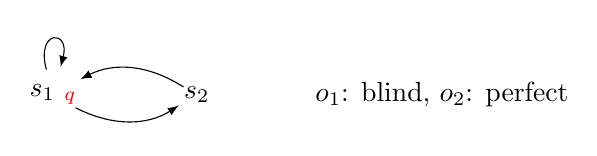
\begin{tikzpicture}[%
      every node/.style={circle,minimum size=4pt,minimum height=4pt, inner sep=0pt},
      shorten >=2pt,
      node distance=1.3cm, >=latex
    ]
    \node [] (0) [circle] {$s_1~_{\color{red}q}$};
    \node [] (1) [circle, right=of 0] {$s_2$};
    \node [] (2) [rectangle, right=of 1] {$o_1$: blind, $o_2$: perfect}; 
    \path [draw] (0) edge[->, bend right]  node {} (1)
    (0) edge[->, loop above]  node {} (0)
    (1) edge[->, bend right]  node {} (0);
  \end{tikzpicture}
  \end{center}
  \hrule
  \begin{center}
  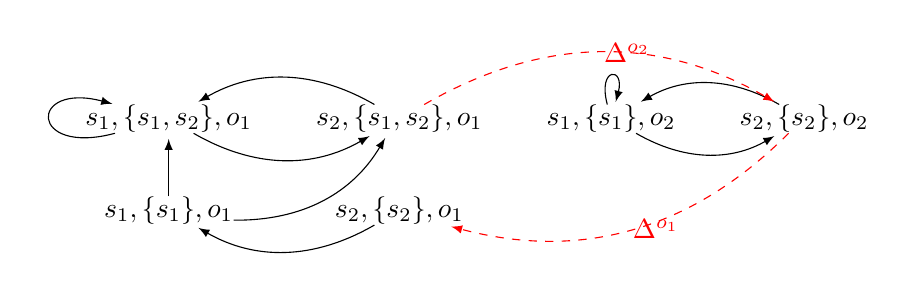
\begin{tikzpicture}[%
      every node/.style={circle,minimum size=4pt,minimum height=4pt, inner sep=0pt},
      shorten >=2pt,
      node distance=0.8cm, >=latex
    ]
    \node [] (0) [rectangle] {$s_1,\{s_1,s_2\},o_1$};
    \node [] (1) [rectangle, right=of 0] {$s_2,\{s_1,s_2\},o_1$};
    \node [] (2) [rectangle, below=of 0] {$s_1,\{s_1\},o_1$};
    \node [] (3) [rectangle, below=of 1] {$s_2,\{s_2\},o_1$};
    \node [] (4) [rectangle, right=of 1] {$s_1,\{s_1\},o_2$};
    \node [] (5) [rectangle, right=of 4] {$s_2,\{s_2\},o_2$};
    \path [draw] (0) edge[->, bend right]  node {} (1)
    (0) edge[->, loop left]  node {} (0)
    (1) edge[->, bend right]  node {} (0)
    (4) edge[->, bend right]  node {} (5)
    (4) edge[->, loop above]  node {} (4)
    (5) edge[->, bend right]  node {} (4)
    (2) edge[->]  node {} (0)
    (2) edge[->, bend right]  node {} (1)
    (3) edge[->, bend left]  node {} (2)
    (1) edge[dashed, ->, bend left, color=red,right] node {$\D{o_2}$} (5)
    (5) edge[dashed, ->, bend left, color=red,right] node {$\D{o_1}$} (3)
    ;
  \end{tikzpicture}
  \end{center}
\end{frame}


\begin{frame}{Example}
  $$\varphi=\D{o_2}(\K q\vee\neg q)$$
  \vfill
    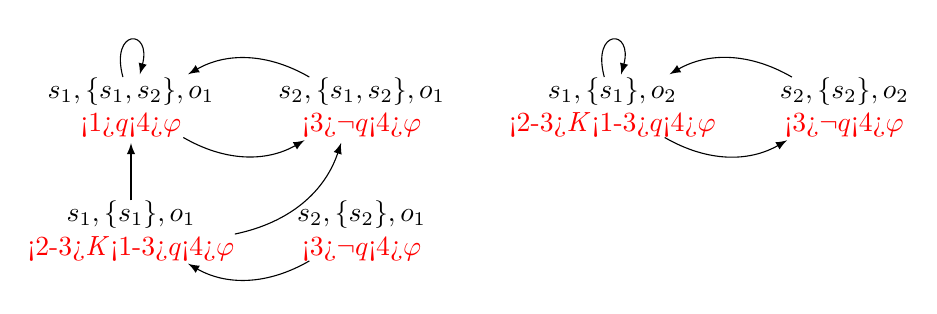
\begin{tikzpicture}[%
      every node/.style={circle,minimum size=4pt,minimum height=4pt, inner sep=0pt},
      shorten >=2pt,
      node distance=0.8cm, >=latex
    ]
    \node [] (0) [rectangle, align=center] {$s_1,\{s_1,s_2\},o_1$\\\color{red}{\onslide<1>{$q$}}{\onslide<4>{$\varphi$}}};
    \node [] (1) [rectangle, right=of 0, align=center] {$s_2,\{s_1,s_2\},o_1$\\\color{red}{\onslide<3>{$\neg q$}}{\onslide<4>{$\varphi$}}};
    \node [] (2) [rectangle, below=of 0, align=center] {$s_1,\{s_1\},o_1$\\\color{red}{\onslide<2-3>{$\K$}}{\onslide<1-3>{$q$}}{\onslide<4>{$\varphi$}}};
    \node [] (3) [rectangle, below=of 1, align=center] {$s_2,\{s_2\},o_1$\\\color{red}{\onslide<3>{$\neg q$}}{\onslide<4>{$\varphi$}}};
    \node [] (4) [rectangle, right=of 1, align=center] {$s_1,\{s_1\},o_2$\\\color{red}{\onslide<2-3>{$\K$}}{\onslide<1-3>{$q$}}{\onslide<4>{$\varphi$}}};
    \node [] (5) [rectangle, right=of 4, align=center] {$s_2,\{s_2\},o_2$\\\color{red}{\onslide<3>{$\neg q$}}{\onslide<4>{$\varphi$}}};
    \path [draw] (0) edge[->, bend right]  node {} (1)
    (0) edge[->, loop above]  node {} (0)
    (1) edge[->, bend right]  node {} (0)
    (4) edge[->, bend right]  node {} (5)
    (4) edge[->, loop above]  node {} (4)
    (5) edge[->, bend right]  node {} (4)
    (2) edge[->]  node {} (0)
    (2) edge[->, bend right]  node {} (1)
    (3) edge[->, bend left]  node {} (2)
    ;
  \end{tikzpicture}
    \vfill
    \textbf{Subformula:}
    \onslide<4>{$\D{o_2}($}\onslide<2,4>{$\K$}\onslide<1-2,4>{$q$}\onslide<4>{$\vee$}\onslide<3-4>{$\neg q$}\onslide<4>{$)$}\\
    
\end{frame}


\begin{frame}{Algorithm}
  \footnotesize
  \begin{block}{While there exists $\D{o}\varphi$ or $\K\varphi$ subformula ($\varphi$ \ctls\ formula)}
    Mark the states where $\varphi$ holds using a \ctls\ model-checker, with a new atomic proposition $p_{\varphi}$.\\
    If the subformula is $\K\varphi$, mark with a new atomic proposition $p_\phi$ every $(I,s,o)$ such that $\forall s'\in I, (I,s',o)$ has been marked with $p_{\varphi}$.\\
    If the subformula is $\D{o}\varphi$, mark with a new atomic proposition $p_\phi$ every $(I,s,o')$ such that $(\UD(I,s,o),s,o)$ has been marked with $p_{\varphi}$.\\
    Replace $\K\varphi$ or $\D{o}\varphi$ with $p_\phi$.
  \end{block}
  \vfill
  \begin{exampleblock}{When there is no more $\K$ or $\D{o}$}
    The final formula is a \ctls\ formula with new atomic propositions.
    It can be model-checked with a \ctls\ model-checker.
  \end{exampleblock}
    

\end{frame}



%\metroset{sectionpage=none}
\section{Conclusion}
\begin{frame}{Multi agent setting}
  \begin{block}{New syntax}
    \begin{tabular}{r l}
    History Formula: & $\varphi := p ~|~ \neg \varphi ~|~ \varphi\wedge\varphi ~|~ \A\psi ~|~ \K_a\varphi ~|~ \D{o}_a\varphi$\\
    Path Formula: & $\psi := \varphi ~|~ \neg\psi ~|~ \psi\wedge\psi ~|~ \X\psi ~|~ \psi\U\psi$
    \end{tabular}
    
    $a$ agent.
  \end{block}
  \vfill
  \begin{block}{\ktrees}
    \begin{center}
      \begin{tikzpicture}[%
      every node/.style={circle,minimum size=4pt,minimum height=4pt, inner sep=0pt},
      shorten >=2pt,
      node distance=1.3cm, >=latex
    ]
        \node [] (0) [circle] {$s_1$};
        \node [] (4) [circle, below left=of 0,xshift=-2cm] {,};
    \node [] (1) [circle, left=of 4,xshift=1cm] {$\{~s_1$};
    \node [] (2) [circle, right=of 4,xshift=-1cm] {$s_2~\}$};
    \node [] (3) [circle, below right=of 0,xshift=2cm] {$\{\quad s_1\quad\}$};
    \node [] (11) [circle, below left=of 1] {$\{s_1\}$};
    \node [] (12) [circle, below=of 1] {$\{s_1\}$};11
    \node [] (21) [circle, below=of 2] {$\{s_2\}$};
    \node [] (22) [circle, below right=of 2] {$\{s_2\}$};    
    \node [] (31) [circle, below left=of 3] {$\{s_1,s_2\}$};
    \node [] (32) [circle, below right=of 3] {$\{s_1\}$};    

    \path
    (0) edge[->,above left]  node {\tiny 1} (4)
    (0) edge[->,above right]  node {\tiny 2} (3)
    (1) edge[->,above left] node {\tiny 1} (11)
    (1) edge[->,right] node {\tiny 2} (12)
    (2) edge[->,left] node {\tiny 1} (21)
    (2) edge[->,above right] node {\tiny 2} (22)
    (3) edge[->,above left] node {\tiny 1} (31)
    (3) edge[->,above right] node {\tiny 2} (32)
    ;
      \end{tikzpicture}
    \end{center}
  \end{block}

\end{frame}


\begin{frame}{Summary}

  \begin{exampleblock}{Definition of \ctlskd}
    First one to study changes of observations with epistemic operators.
  \end{exampleblock}
  \vfill
  \begin{exampleblock}{Definition of alternative semantics}
    Easier to model-check.\\
    Proved the equivalence between the two semantics.
  \end{exampleblock}
  \vfill
  \begin{exampleblock}{Model-Checking}
    Marking Algorithm.\\
    EXPTIME for single-agent setting.
  \end{exampleblock}
  \vfill
  \begin{exampleblock}{Multi-agent setting}
    Nonelementary complexity for model-checking.
  \end{exampleblock}
   
\end{frame}


\begin{frame}{Future Works}

  \begin{itemize}
  \item Extend the logic. Allow $\D{o}$ in path formulas.
  \item Axiomatization of \ctlskd.
  \item Implementation of the Model-Checking Algorithm.
  \item Epistemic Extension of Strategy Logic with Imperfect Information.
  \end{itemize}
  
\end{frame}


\end{document}
